%% =============================================================
%% SecureZone - Major Project Proposal
%% Overleaf Compatible | IEEE Conference Style
%% =============================================================
\documentclass[conference]{IEEEtran}

% ===== Packages =====
\usepackage{cite}
\usepackage{amsmath,amssymb,amsfonts}
\usepackage{algorithmic}
\usepackage{graphicx}
\usepackage{textcomp}
\usepackage{xcolor}
\usepackage{hyperref}
\usepackage{booktabs}
\usepackage{tabularx}
\usepackage{enumitem}
\usepackage{tikz}
\usetikzlibrary{shapes.geometric, arrows.meta, positioning, fit}

% ===== Metadata =====
\hypersetup{
    colorlinks=true,
    linkcolor=blue,
    citecolor=blue,
    urlcolor=blue,
}

\begin{document}

% =============================================================
% TITLE
% =============================================================
\title{SecureZone: A Proximity-Based Zero-Trust Architecture for Continuous File Encryption and Physical Access Control}

% =============================================================
% AUTHORS — Replace placeholders
% =============================================================
\author{
    \IEEEauthorblockN{
        \textbf{Student Name 1}\textsuperscript{1},
        \textbf{Student Name 2}\textsuperscript{2},
        \textbf{Student Name 3}\textsuperscript{3}
        % Add/remove students as needed
    }
    \IEEEauthorblockA{
        \textsuperscript{1,2,3}Department of \textit{<<Your Department>>},\\
        \textit{<<Your College/University Name>>},\\
        \textit{<<City, State, Country>>}\\
        \textsuperscript{1}\texttt{<<email1@college.edu>>},
        \textsuperscript{2}\texttt{<<email2@college.edu>>},
        \textsuperscript{3}\texttt{<<email3@college.edu>>}
    }
    \\[1em]
    \IEEEauthorblockN{\textbf{Project Guide:} Prof. <<Guide Name>>}
    \IEEEauthorblockA{
        Department of \textit{<<Department>>},\\
        \textit{<<College/University Name>>}\\
        \texttt{<<guide.email@college.edu>>}
    }
}

\maketitle

% =============================================================
% ABSTRACT
% =============================================================
\begin{abstract}
Insider threats and unauthorized data exfiltration pose significant risks to corporate networks. Traditional Data Loss Prevention (DLP) systems rely on perimeter defense or manual device confiscation, both of which are prone to human error and degrade user experience. This proposal presents \textbf{SecureZone}, a Zero-Trust physical-digital bridge system that utilizes wearable IoT badges based on ESP32 Bluetooth Low Energy (BLE) to continuously authenticate users based on physical proximity to a workstation. Protected files remain heavily encrypted using AES-256-GCM at rest and are only temporarily decrypted into volatile memory (RAM) when an authorized badge is detected within a defined 2-meter spatial radius. The system integrates Role-Based Access Control (RBAC), ephemeral cryptographic key management, and a fail-closed security architecture to ensure data remains mathematically unreadable when removed from the authorized physical premises or when the authorized user steps away from the terminal.
\end{abstract}

\begin{IEEEkeywords}
Zero-Trust Architecture, Bluetooth Low Energy (BLE), IoT Security, AES-256-GCM, Proximity Authentication, Data Loss Prevention, RBAC, Continuous Authentication, ESP32
\end{IEEEkeywords}

% =============================================================
% 1. INTRODUCTION
% =============================================================
\section{Introduction}

The proliferation of digital data within organizations has made data protection a paramount concern. While external cybersecurity threats receive significant attention, insider threats—whether malicious or accidental—account for a substantial proportion of data breaches \cite{verizon2023}. Current organizational security models struggle to prevent data theft by authorized personnel or physically present malicious actors. Once a file is downloaded to a local machine or copied to an external storage device, the organization effectively loses control over that data.

Traditional Data Loss Prevention (DLP) solutions operate at the network perimeter or endpoint level, employing techniques such as content inspection, device control policies, and network monitoring \cite{dlp_survey}. However, these approaches suffer from fundamental limitations: they cannot prevent an authorized user from simply walking away with sensitive data on a USB drive, nor can they enforce access policies based on the user's real-time physical location.

\subsection{Motivation}
There exists a critical gap between digital access control and physical security. A user who is authenticated once at login retains access for the entire session, regardless of whether they remain at their workstation. This ``authenticate once, access forever'' paradigm violates the core principles of Zero-Trust security, which mandate continuous verification \cite{nist_zerotrust}.

\subsection{Proposed Solution}
This project proposes \textbf{SecureZone}, a system that \textit{inextricably links} digital access rights to verifiable, continuous physical presence within a highly restricted area. Through the use of ESP32-based BLE wearable badges, AES-256-GCM file encryption, and ephemeral key management, SecureZone ensures that:
\begin{itemize}[noitemsep]
    \item Files are \textbf{always encrypted at rest} on the workstation.
    \item Decryption occurs \textbf{only in volatile memory} (RAM-backed tmpfs), never touching persistent storage.
    \item The decryption key is \textbf{immediately wiped} the moment the authorized user steps beyond a 2-meter radius.
    \item Copied or exfiltrated files are \textbf{mathematically unreadable} without the server-held master key.
\end{itemize}

% =============================================================
% 2. LITERATURE REVIEW
% =============================================================
\section{Literature Review}

\subsection{Zero-Trust Architecture}
The Zero-Trust model, formalized by NIST in SP 800-207 \cite{nist_zerotrust}, operates on the principle of ``never trust, always verify.'' Unlike traditional perimeter-based security, Zero-Trust requires continuous authentication and authorization for every access request, regardless of the user's location within or outside the network boundary.

\subsection{BLE-Based Proximity Detection}
Bluetooth Low Energy (BLE) has been widely adopted for indoor proximity estimation due to its low power consumption and ubiquitous hardware support. Received Signal Strength Indicator (RSSI) is the primary metric for distance estimation in BLE systems \cite{ble_rssi_survey}. However, RSSI measurements are inherently noisy due to multipath propagation, body shielding, and environmental interference. Kalman filtering and Exponential Moving Average (EMA) techniques have been shown to significantly improve RSSI-based distance accuracy \cite{kalman_ble}.

\subsection{Transparent File Encryption}
Full-disk encryption solutions such as BitLocker and LUKS protect data at rest but offer no file-level granularity or proximity-based access control \cite{fde_survey}. Application-layer encryption libraries such as the Python \texttt{cryptography} module provide AES-256-GCM, which offers both confidentiality and integrity through authenticated encryption \cite{aes_gcm_nist}.

\subsection{Data Loss Prevention}
Existing DLP systems rely on content inspection, device whitelisting, and network monitoring \cite{dlp_survey}. These systems cannot prevent an authorized user from copying encrypted files to removable media and later extracting them outside the monitored environment. SecureZone addresses this gap by ensuring that the decryption key is ephemeral and spatially bound.

% =============================================================
% 3. RESEARCH OBJECTIVES
% =============================================================
\section{Research Objectives}

The primary objectives of this research are:

\begin{enumerate}[noitemsep]
    \item \textbf{Design a Continuous Authentication Mechanism:} Engineer an ESP32-based IoT smart badge that emits continuous BLE proximity signals to a workstation receiver node, with RSSI-based distance estimation enhanced by Kalman filtering and hysteresis thresholding.

    \item \textbf{Implement Proximity-Dependent Cryptography:} Develop a background operating system agent that executes transparent AES-256-GCM encryption/decryption on local files, fetching ephemeral decryption keys from a central server only when the authorized badge is within a 2-meter radius.

    \item \textbf{Develop a Hierarchical RBAC Backend:} Create a centralized server architecture that maps badge IDs to specific device IDs, enforcing access rules across a three-tier hierarchy: Administrator, Manager, and Employee.

    \item \textbf{Implement Fail-Closed Security:} Ensure the system defaults to a locked state under all failure conditions—server outage, badge absence, or network disruption—guaranteeing that no data is accessible without active, verified authorization.

    \item \textbf{Establish Audit Logging and Monitoring:} Implement a comprehensive logging dashboard for monitoring access timestamps, badge proximity events, and security incidents.
\end{enumerate}

% =============================================================
% 4. SYSTEM ARCHITECTURE
% =============================================================
\section{Proposed System Architecture}

The SecureZone system consists of four primary components operating across three layers, as illustrated in Fig.~\ref{fig:architecture}.

\begin{figure}[htbp]
    \centering
    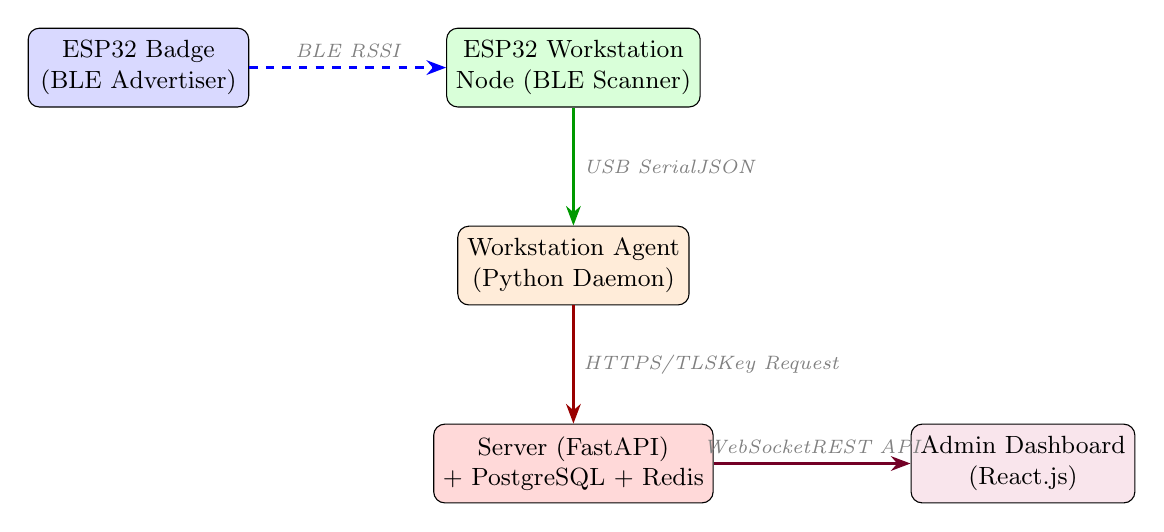
\begin{tikzpicture}[
        node distance=1.2cm and 2cm,
        block/.style={rectangle, draw, rounded corners, minimum width=2.8cm, minimum height=1cm, align=center, font=\small},
        arrow/.style={-{Stealth[length=2.5mm]}, thick},
        label/.style={font=\scriptsize\itshape, text=gray}
    ]
        % Nodes
        \node[block, fill=blue!15] (badge) {ESP32 Badge\\(BLE Advertiser)};
        \node[block, fill=green!15, right=2.5cm of badge] (anchor) {ESP32 Workstation\\Node (BLE Scanner)};
        \node[block, fill=orange!15, below=1.5cm of anchor] (agent) {Workstation Agent\\(Python Daemon)};
        \node[block, fill=red!15, below=1.5cm of agent] (server) {Server (FastAPI)\\+ PostgreSQL + Redis};
        \node[block, fill=purple!10, right=2.5cm of server] (dashboard) {Admin Dashboard\\(React.js)};

        % Arrows
        \draw[arrow, dashed, blue] (badge) -- node[above, label] {BLE RSSI} (anchor);
        \draw[arrow, green!60!black] (anchor) -- node[right, label] {USB Serial\\JSON} (agent);
        \draw[arrow, red!60!black] (agent) -- node[right, label] {HTTPS/TLS\\Key Request} (server);
        \draw[arrow, purple!60!black] (server) -- node[above, label] {WebSocket\\REST API} (dashboard);
    \end{tikzpicture}
    \caption{High-level system architecture of SecureZone showing the four primary components and their communication protocols.}
    \label{fig:architecture}
\end{figure}

\subsection{Hardware Layer}
\begin{itemize}[noitemsep]
    \item \textbf{Smart Badge (ESP32-WROOM-32):} A battery-powered wearable device that continuously broadcasts BLE advertisements containing a rotating encrypted nonce and a unique badge identifier. Deep-sleep cycling (100ms advertise / 400ms sleep) optimizes battery life.
    \item \textbf{Workstation Receiver Node (ESP32-WROOM-32):} A USB-connected BLE scanner that detects nearby badges, measures RSSI, and forwards proximity data as JSON over USB Serial to the host agent.
\end{itemize}

\subsection{Signal Processing Layer}
Raw BLE RSSI values are inherently noisy. The system employs a multi-stage filtering pipeline:
\begin{enumerate}[noitemsep]
    \item \textbf{Exponential Moving Average (EMA):} Smooths raw RSSI with $\alpha = 0.3$ to dampen transient spikes.
    \item \textbf{Kalman Filter:} Predicts steady-state RSSI and rejects noise from body shielding and multipath reflections.
    \item \textbf{Hysteresis Thresholding:} Authorizes at RSSI $\geq -63$ dBm and de-authorizes at RSSI $\leq -68$ dBm, preventing rapid toggling at the boundary.
    \item \textbf{Grace Period:} Requires 5 consecutive out-of-range readings ($\approx$2.5s) before triggering key revocation.
\end{enumerate}

\subsection{Cryptographic Layer}
\begin{itemize}[noitemsep]
    \item \textbf{AES-256-GCM:} All protected files are encrypted using AES-256 in Galois/Counter Mode, providing both confidentiality and integrity verification.
    \item \textbf{Ephemeral Key Exchange:} File Encryption Keys (FEKs) are never stored locally. The agent requests short-lived keys (TTL = 60s) from the server over TLS 1.3, only when an authorized badge is within range.
    \item \textbf{RAM-backed Decryption:} Decrypted content is written exclusively to a \texttt{tmpfs} mount, ensuring it never touches persistent storage.
    \item \textbf{Secure Key Wiping:} Upon badge departure, FEKs are overwritten with zeros in memory and the tmpfs mount is unmounted.
\end{itemize}

\subsection{Backend and Administrative Layer}
\begin{itemize}[noitemsep]
    \item \textbf{FastAPI Server:} Handles badge authentication, key distribution, RBAC enforcement, and audit logging.
    \item \textbf{PostgreSQL Database:} Stores user-badge-device mappings, access policies, file key metadata, and audit logs.
    \item \textbf{Redis Cache:} Provides fast ephemeral key storage with automatic TTL-based expiration.
    \item \textbf{Admin Dashboard:} A React.js web application for badge management, access policy configuration, and real-time audit log monitoring.
\end{itemize}

% =============================================================
% 5. METHODOLOGY
% =============================================================
\section{Methodology}

The project follows an incremental development methodology with a clearly defined MVP (Minimum Viable Product) scope.

\subsection{MVP Scope}
The MVP focuses exclusively on the core security loop:
\begin{enumerate}[noitemsep]
    \item BLE badge detection with RSSI filtering
    \item AES-256-GCM file encryption/decryption
    \item Ephemeral key exchange (badge in range $\rightarrow$ key $\rightarrow$ decrypt in RAM)
    \item Automatic key wipe on badge exit
    \item Server-side RBAC and audit logging
    \item Fail-closed agent behavior
\end{enumerate}

\subsection{Development Phases}
\begin{table}[htbp]
    \centering
    \caption{Project Development Timeline}
    \label{tab:timeline}
    \begin{tabularx}{\columnwidth}{l l X}
        \toprule
        \textbf{Phase} & \textbf{Duration} & \textbf{Deliverable} \\
        \midrule
        0. Setup & Week 1--2 & Hardware procurement, environment setup, repository scaffold \\
        1. IoT/BLE & Week 3--5 & Badge \& anchor firmware, RSSI calibration with Kalman filter \\
        2. Crypto Engine & Week 5--8 & Agent daemon, AES-256-GCM encrypt/decrypt, fail-closed mode \\
        3. Backend & Week 7--10 & FastAPI server, RBAC, key management, audit logs \\
        4. Dashboard & Week 9--11 & Admin web portal with badge management \& logs \\
        5. Testing & Week 11--13 & Integration, security, and performance testing \\
        6. Documentation & Week 13--15 & IEEE paper, demo video, presentation \\
        \bottomrule
    \end{tabularx}
\end{table}

\subsection{Risk Mitigation}
\begin{table}[htbp]
    \centering
    \caption{Identified Risks and Mitigation Strategies}
    \label{tab:risks}
    \begin{tabularx}{\columnwidth}{l X}
        \toprule
        \textbf{Risk} & \textbf{Mitigation} \\
        \midrule
        BLE RSSI unreliability & Kalman filter + EMA + hysteresis + grace period; wired USB-serial fallback mode \\
        Scope creep & Strict MVP/Post-MVP split; no Post-MVP work until core loop verified \\
        Server single point of failure & Fail-closed agent: instant key wipe, lockdown, re-auth on reconnect \\
        \bottomrule
    \end{tabularx}
\end{table}

% =============================================================
% 6. EXPECTED OUTCOMES
% =============================================================
\section{Expected Outcomes}

The final deliverable will be a working prototype demonstrating a seamless Zero-Trust environment. Specifically:

\begin{enumerate}[noitemsep]
    \item Files on the workstation remain encrypted (AES-256-GCM) at all times on disk.
    \item When an authorized badge is within 2 meters, files are transparently decrypted into RAM for user access.
    \item The moment the badge exits the 2-meter radius, all decryption keys are wiped and files become unreadable within 5 seconds.
    \item Files copied to a USB drive or saved externally are entirely inaccessible, as only the encrypted ciphertext is ever written to persistent storage.
    \item If the server becomes unreachable, the agent locks all files immediately (fail-closed).
    \item All access events are logged with timestamps, badge IDs, and RSSI values for forensic analysis.
\end{enumerate}

% =============================================================
% 7. HARDWARE & SOFTWARE REQUIREMENTS
% =============================================================
\section{Hardware and Software Requirements}

\subsection{Hardware}
\begin{table}[htbp]
    \centering
    \caption{Hardware Components}
    \label{tab:hardware}
    \begin{tabularx}{\columnwidth}{l c X}
        \toprule
        \textbf{Component} & \textbf{Qty} & \textbf{Purpose} \\
        \midrule
        ESP32-WROOM-32 & 3 & 2 badges + 1 workstation node \\
        Li-Po Battery (500mAh) & 2 & Badge power supply \\
        USB Cables & 3 & Development \& serial communication \\
        Breadboard & 1 & Prototyping \\
        \bottomrule
    \end{tabularx}
\end{table}

\subsection{Software}
\begin{table}[htbp]
    \centering
    \caption{Software Stack}
    \label{tab:software}
    \begin{tabularx}{\columnwidth}{l X}
        \toprule
        \textbf{Layer} & \textbf{Technology} \\
        \midrule
        IoT Firmware & Arduino IDE / PlatformIO (ESP-IDF) \\
        Host Agent & Python 3.11+ (bleak, cryptography, watchdog) \\
        Backend Server & Python FastAPI, SQLAlchemy, Alembic \\
        Database & PostgreSQL 15+ \\
        Key Cache & Redis 7+ \\
        IoT Messaging & MQTT (Mosquitto) \\
        Admin Dashboard & React.js, Vite, WebSocket \\
        Encryption & AES-256-GCM (Python cryptography lib) \\
        \bottomrule
    \end{tabularx}
\end{table}

% =============================================================
% 8. CONCLUSION
% =============================================================
\section{Conclusion}

This proposal presents SecureZone, a novel proximity-based Zero-Trust system that addresses the critical gap between digital access control and physical security. By combining BLE-based continuous proximity authentication with AES-256-GCM file encryption and ephemeral key management, the system ensures that sensitive data is mathematically inaccessible outside the authorized physical zone. The fail-closed architecture guarantees security under all failure conditions, while the signal processing pipeline (EMA, Kalman filter, hysteresis) ensures reliable proximity detection despite inherent BLE RSSI noise. The proposed system has direct applicability in defense installations, financial institutions, healthcare facilities, and any environment where physical data exfiltration is a critical threat.

% =============================================================
% REFERENCES
% =============================================================
\begin{thebibliography}{00}

\bibitem{verizon2023}
Verizon, ``2023 Data Breach Investigations Report,'' Verizon Business, 2023. [Online]. Available: \url{https://www.verizon.com/business/resources/reports/dbir/}

\bibitem{nist_zerotrust}
S. Rose, O. Borchert, S. Mitchell, and S. Connelly, ``Zero Trust Architecture,'' NIST Special Publication 800-207, National Institute of Standards and Technology, Aug. 2020.

\bibitem{dlp_survey}
A. Shabtai, Y. Elovici, and L. Rokach, ``A Survey of Data Leakage Detection and Prevention Solutions,'' Springer Briefs in Computer Science, 2012.

\bibitem{ble_rssi_survey}
F. Zafari, A. Gkelias, and K. K. Leung, ``A Survey of Indoor Localization Systems and Technologies,'' \textit{IEEE Communications Surveys \& Tutorials}, vol. 21, no. 3, pp. 2568--2599, 2019.

\bibitem{kalman_ble}
R. Faragher and R. Harle, ``Location Fingerprinting With Bluetooth Low Energy Beacons,'' \textit{IEEE Journal on Selected Areas in Communications}, vol. 33, no. 11, pp. 2418--2428, Nov. 2015.

\bibitem{fde_survey}
N. Ferguson, B. Schneier, and T. Kohno, ``Cryptography Engineering: Design Principles and Practical Applications,'' Wiley, 2010.

\bibitem{aes_gcm_nist}
M. Dworkin, ``Recommendation for Block Cipher Modes of Operation: Galois/Counter Mode (GCM) and GMAC,'' NIST Special Publication 800-38D, Nov. 2007.

\end{thebibliography}

\end{document}
